\section{Results}
\label{sec:results}
The results follow the endpoints: first the tail damage per class, then its split into own and other-class loss, the rank response with the additivity check, and finally the class properties. The balanced arm reaches 39.57 percent balanced accuracy (36.70 to 42.53), as in the prevalence curve. Averaged over the seven classes, the tail damage is 4.18 points (3.20 to 5.29) at $\rho=10$ and 7.87 points (6.60 to 9.27) at $\rho=100$, slightly above the 4.02 and 7.65 points of the prevalence study. The difference comes from the reused shift 0: at $\rho=100$ the seven shifts reach between 30.99 and 32.21 percent balanced accuracy, and shift 0, at 31.92 percent, lies above their mean of 31.70.

\subsection{Tail damage per class}
\label{sec:damage-results}
Which class sits in the tail changes the damage materially (Table~\ref{tab:damage}, Figure~\ref{fig:damage}). At $\rho=100$ the damage ranges from 5.73 points with UDH in the tail and 5.77 points with ADH to 9.37 points with N and 9.99 points with IC, a spread of 4.3 points with a standard deviation of 1.56 points across classes. The intervals of the two extremes do not overlap. At $\rho=10$ the damage ranges from 2.56 points with ADH to 5.46 points with N, a spread of 2.9 points with a standard deviation of 1.15 points. Both spreads exceed the one-point threshold, although, as stated in Section~\ref{sec:evaluation}, the spread between the extremes of seven means overstates the true spread.

\begin{table}[htbp]
\centering
\renewcommand{\arraystretch}{1.15}
\begin{tabular}{@{}lrrll@{}}
\toprule
Tail class & r1 recall & Confusability & $D_{10}(c)$ & $D_{100}(c)$ \\
\midrule
ADH & 12.23 & 7.4 & 2.56 [1.19, 4.16] & 5.77 [4.06, 7.69] \\
UDH & 22.98 & 11.4 & 2.97 [1.62, 4.34] & 5.73 [3.93, 7.52] \\
PB & 31.42 & 23.7 & 3.09 [1.60, 4.67] & 7.25 [5.26, 9.44] \\
DCIS & 36.19 & 9.2 & 5.06 [3.59, 6.67] & 8.23 [6.42, 10.05] \\
FEA & 44.62 & 9.0 & 5.31 [3.67, 6.97] & 8.76 [6.71, 11.00] \\
N & 60.47 & 16.3 & 5.46 [3.95, 7.13] & 9.37 [7.54, 11.32] \\
IC & 69.07 & 6.3 & 4.79 [3.30, 6.29] & 9.99 [8.26, 11.80] \\
\addlinespace
Mean & 39.57 & & 4.18 [3.20, 5.29] & 7.87 [6.60, 9.27] \\
\bottomrule
\end{tabular}
\caption{The damage grows with the balanced-arm recall of the class in the tail. Tail damage $D_\rho(c)$ is the balanced-accuracy loss against the balanced arm, in points with paired 95\% bootstrap intervals, over the 30 fits in which class $c$ occupies the tail. Classes are ordered by their patient-macro recall in the balanced arm, in percent; confusability is the off-diagonal confusion mass into and out of the class in percent of all balanced-arm test predictions.}
\label{tab:damage}
\end{table}

\noindent The ordering does not follow the overlap reading, under which the hardest classes would cost the most. ADH and UDH, the two classes with the lowest balanced recall, are the cheapest tail classes at both ratios. Instead, the ordering follows the balanced-arm recall. The Spearman correlation between r1 recall and tail damage is 0.79 at $\rho=10$ and 0.96 at $\rho=100$, where only UDH and ADH swap places. The correlation with confusability is 0.18 and $-0.29$.

\begin{figure}[htbp]
\centering
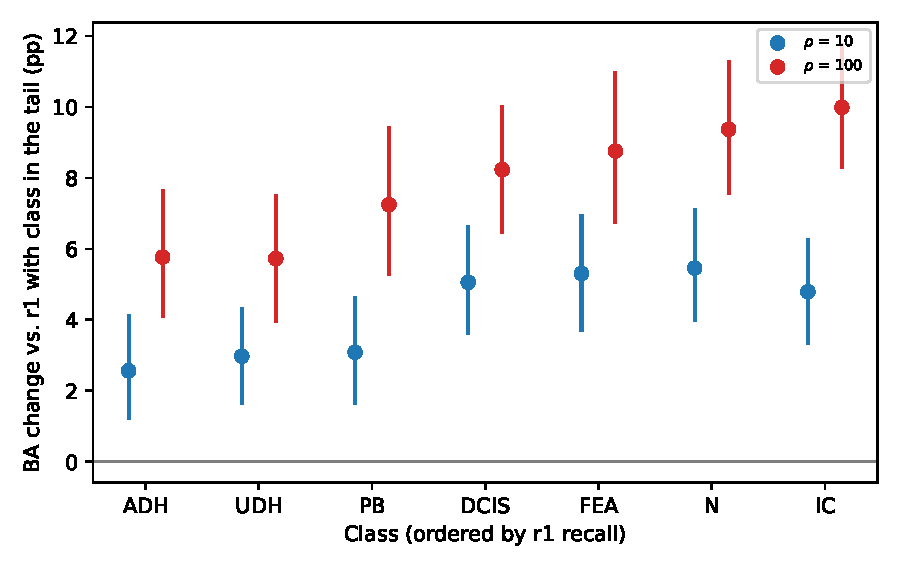
\includegraphics[width=0.7\textwidth]{tail_damage.pdf}
\caption{Easy classes cost the most when they sit in the tail. Balanced-accuracy loss against the balanced arm, in points, with the class on the horizontal axis placed in the tail, at $\rho=10$ (blue) and $\rho=100$ (red), with paired 95\% bootstrap intervals. Classes are ordered by their recall in the balanced arm, from ADH (12 percent) to IC (69 percent).}
\label{fig:damage}
\end{figure}

\subsection{Own loss and loss on the other classes}
\label{sec:split-results}
Most of the tail damage is the tail class's own lost recall (Table~\ref{tab:split}). At $\rho=100$, six of the seven classes keep at most 4 percent recall in the tail: ADH 1.1, UDH 0.9, PB 3.3, DCIS 2.1, FEA 1.6, and N 3.9 percent. Each of them thus loses between 89 and 96 percent of its balanced recall, and its own loss is close to its balanced recall divided by seven. Only IC keeps 34.0 percent, half of its 69.1 percent. At $\rho=10$ the collapse is less complete and depends on the class: ADH keeps 1.6 percent, whereas FEA keeps 14.4, N 18.5, and IC 50.5 percent. Averaged over classes, the own loss is 3.43 of the 4.18 points at $\rho=10$, 82 percent, and 4.70 of the 7.87 points at $\rho=100$, 60 percent.

\begin{table}[htbp]
\centering
\small
\setlength{\tabcolsep}{4pt}
\renewcommand{\arraystretch}{1.15}
\begin{tabular}{@{}lrrrrrlrl@{}}
\toprule
 & \multicolumn{2}{c}{Tail recall} & \multicolumn{3}{c}{Own loss} & \multicolumn{3}{c}{Loss on other classes} \\
\cmidrule(lr){2-3}\cmidrule(lr){4-6}\cmidrule(lr){7-9}
Tail class & $\rho=10$ & $\rho=100$ & $\rho=10$ & \multicolumn{2}{l}{$\rho=100$} & $\rho=10$ & \multicolumn{2}{l}{$\rho=100$} \\
\midrule
ADH & 1.6 & 1.1 & 1.52 & 1.60 & [1.05, 2.31] & 1.05 & 4.17 & [2.50, 6.14] \\
UDH & 5.7 & 0.9 & 2.47 & 3.16 & [2.45, 3.94] & 0.50 & 2.57 & [0.70, 4.51] \\
PB & 11.0 & 3.3 & 2.91 & 4.01 & [2.99, 5.13] & 0.17 & 3.23 & [1.31, 5.46] \\
DCIS & 7.2 & 2.1 & 4.14 & 4.87 & [3.65, 6.14] & 0.92 & 3.37 & [1.72, 5.08] \\
FEA & 14.4 & 1.6 & 4.32 & 6.15 & [4.99, 7.46] & 0.99 & 2.61 & [1.06, 4.26] \\
N & 18.5 & 3.9 & 5.99 & 8.08 & [6.82, 9.30] & $-$0.53 & 1.30 & [$-$0.60, 3.31] \\
IC & 50.5 & 34.0 & 2.65 & 5.01 & [4.08, 6.02] & 2.14 & 4.98 & [3.33, 6.70] \\
\bottomrule
\end{tabular}
\caption{In the tail at $\rho=100$ every class except IC loses almost all of its recall, so its own loss tracks its balanced recall. Tail recall is the mean own patient-macro recall of the class in percent when it occupies the tail. The own loss is the drop of that recall against the balanced arm divided by seven, the share of balanced accuracy it removes; the loss on the other classes is the rest of $D_\rho(c)$. Both are in points, with paired 95\% bootstrap intervals at $\rho=100$; the $\rho=10$ intervals of the other-class loss contain zero for every class except IC (0.74 to 3.61).}
\label{tab:split}
\end{table}

\noindent The loss on the other classes is small at $\rho=10$, where its interval excludes zero only with IC in the tail, and it grows to between 1.30 and 4.98 points at $\rho=100$. It is largest with IC and ADH in the tail and smallest with N. For ADH, it carries 72 percent of the damage. ADH has little recall of its own to lose, but it is also among the classes that gain most at the upper ranks (Section~\ref{sec:rank-results}); with ADH in the tail, those ranks go to classes that gain less there. Because the arrangement of the other six classes is tied to the tail class within each draw (Section~\ref{sec:design}), these per-class values of the other-class loss are not interpreted further.

\subsection{Rank response and additivity}
\label{sec:rank-results}
Every class responds to its rank in the same monotone way, and the size of the response follows its headroom in both directions (Figure~\ref{fig:rank}). At $\rho=100$ a class at the head gains between 7.5 points of recall (IC) and 37.3 points (UDH); the classes with low balanced recall, UDH, ADH, and PB, gain the most, by 30 to 37 points, while N and IC, which have the least room above them, gain 13.8 and 7.5 points. Toward the tail, the order reverses: N loses 56.5 points and FEA 43.0, while ADH and UDH lose 11.2 and 22.1 points. For the low-recall classes the loss saturates before the tail: ADH loses 11.1 points at rank 5 and 11.2 at rank 6, and it has nothing left to lose beyond. The step from rank 5 to rank 6, where the class count falls from 26 to 12 patches, removes a further 6.3 to 8.3 points from FEA, N, IC, and PB. At rank 3, with 120 patches, the recall of ADH, UDH, and PB is within 3 points of the balanced arm, whereas N already loses 24.8 points and FEA 18.0.

\begin{figure}[htbp]
\centering
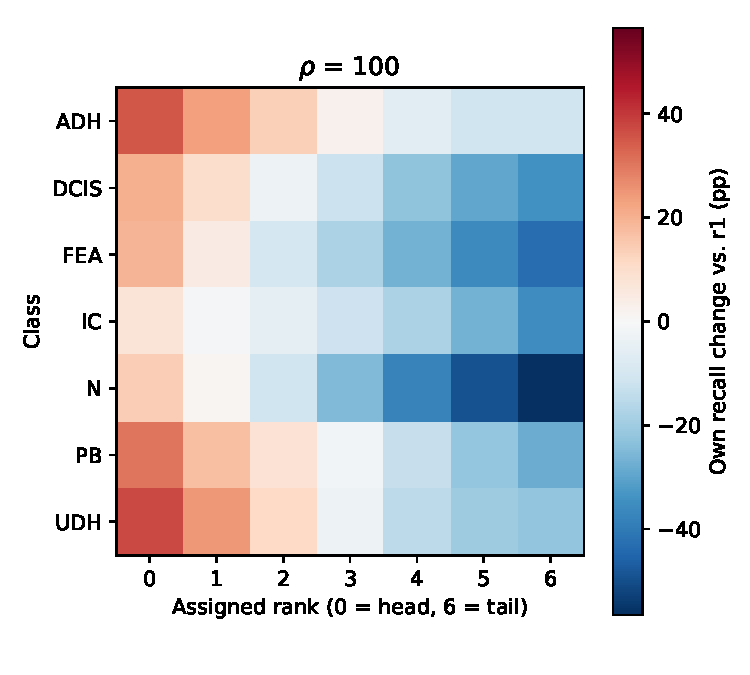
\includegraphics[width=0.6\textwidth]{rank_response_r100.pdf}
\caption{Every class gains recall at the head and loses it toward the tail, and the easy classes N and IC gain least and lose most. Change of each class's own patient-macro recall against the balanced arm, in points, when the class sits at the given rank at $\rho=100$; rank 0 receives 1,206 patches and rank 6 receives 12. Each cell pools the 30 fits in which that class holds that rank.}
\label{fig:rank}
\end{figure}

\noindent The own-rank model explains 73 percent of the variance of the per-fit, per-class recall changes at $\rho=10$ and 79 percent at $\rho=100$. The remaining 27 and 21 percent contain the effect of which other classes hold the other ranks, but also the fit-to-fit variation of per-class recall over test patients and draws, which the design cannot separate from it. The pairings of classes can therefore explain at most about a quarter of the variance, and the damage is largely the sum of the separate responses of the seven classes to their own ranks.

\subsection{Class properties}
\label{sec:properties-results}
Of the two class properties, only the headroom orders the damage. The own loss of the tail class correlates with its balanced recall at 0.64 at $\rho=10$ and 0.89 at $\rho=100$, and with confusability at 0.39 and 0.07. Confusability does not follow balanced recall: PB and N are the most confused classes of the balanced arm, with 23.7 and 16.3 percent of all predictions, while ADH, the class with the lowest recall, lies at 7.4 percent. The least confused class, IC, is the only one that keeps a substantial share of its recall in the tail.

In relative terms, harder classes do collapse faster, as the overlap mechanism predicts, but only at the moderate ratio. At $\rho=10$, ADH loses 87 percent of its balanced recall, DCIS 80 and UDH 75 percent, while FEA, N, and PB lose 65 to 69 percent and IC 27 percent; the Spearman correlation between balanced recall and the lost fraction, computed from Table~\ref{tab:split}, is $-0.68$. At $\rho=100$ all classes except IC lose 89 to 96 percent, and the lost fraction no longer distinguishes them.

\section{Discussion}
\label{sec:discussion}
The class in the tail matters on BRACS: at $\rho=100$ it moves the damage between about 5.7 and 10 points, a range as wide as the prevalence damage at $\rho=10$. The ordering is not the one the difficulty-by-prevalence reading predicts. The hardest classes are the cheapest in the tail, not the most costly. The ordering follows the headroom mechanism instead: at $\rho=100$ nearly every class loses almost all of its recall when it is rare, so the damage a class causes in the tail is set by how much recall it had to lose. IC and N, the classes the balanced classifier recognizes best, cause the largest damage; ADH, which the balanced classifier recognizes in only 12 percent of patients, causes one of the smallest.

The overlap mechanism is not refuted but acts on a different scale. At $\rho=10$ the harder classes lose a larger fraction of their recall than the easy ones, and IC, the most distinct class of the balanced arm, is the only class that survives the tail at $\rho=100$ with half of its recall. Overlap thus decides how fast and how completely a rare class collapses, and headroom decides what this collapse costs in balanced accuracy. On BRACS the collapse is nearly complete for six of seven classes at $\rho=100$, so headroom dominates the damage.

This refines the account of the BRACS damage given by the preceding studies. The prevalence study found a damage seven times that of TCGA-UT \citep{queisler2026prevalenceBracs}, and the prior-versus-support study found that the tail classes fall to a recall floor that further imbalance hardly moves \citep{queisler2026causeBracs}. The present results show that this floor is close to zero for six of the seven classes and not specific to the hard ones. The large BRACS damage therefore does not come from one hard class that happens to be rare; it arises because almost any BRACS class disappears from the predictions once it is rare, whereas the tail third on TCGA-UT keeps about 60 percent recall at $\rho=100$ \citep{queisler2026causeTcga}. The high sensitivity of BRACS to imbalance is a property of the dataset as a whole under ten patients per class, not of a few hard classes.

For the design of imbalance studies, the results support the random class order per draw used throughout this series. A study that fixes one class order on BRACS would report a damage anywhere between about 5.7 and 10 points at $\rho=100$, depending on which class it happened to make rare, and, with $R^2$ values of 0.73 and 0.79 for the own-rank model, most of this variation is predictable from the rank response of each class. Averaging over assignments, as the prevalence study does, estimates the damage for an unknown rare class; the tail damage per class answers the more specific clinical question of what happens when a given lesion type is the rare one.

\section{Limitations}
\label{sec:limitations}
With seven classes, the correlations with class properties rest on seven points and are descriptive; the per-class damages have intervals of about $\pm 1.8$ points, so only the extremes of the ordering are well separated. The Latin square is built from cyclic shifts of one random order per draw, so within a draw the tail class always has the same neighbours at the next ranks; these vary across the 30 draws but are not balanced, and the other-class loss per tail class depends on them. The own-rank model cannot separate the effect of class pairings from fit-to-fit variation, so its $R^2$ gives only a lower bound on additivity.

The confusability measure pools patch-level confusion counts and therefore gives classes with many test patches more weight, and it does not capture overlap as a pathologist would rate it. The study covers two ratios and one exponential profile. All results are conditional on ten patients per class, frozen Virchow2 features, multinomial logistic regression, BRACS, and three overlapping splits with about 24 test patients each.
